%% ======================================================================
%% 08_operation.tex -- 7. Operation instructions
%% ======================================================================
\section{Operation instructions}
\label{sec:operation}

\begin{figure}[!htbp]
  \centering
  \begin{subfigure}[b]{0.52\textwidth}\centering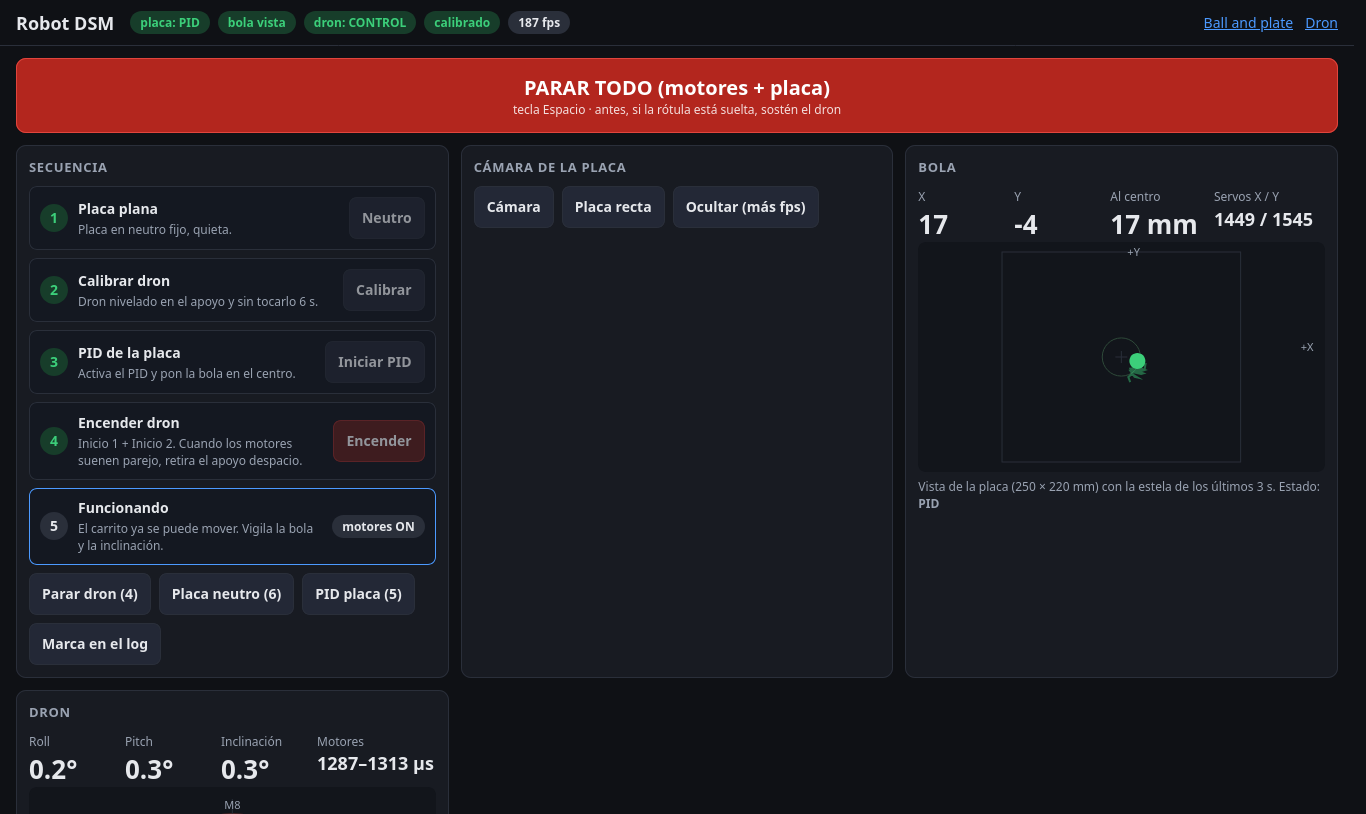
\includegraphics[width=\linewidth]{figures/ui_robot_page.png}\caption{\texttt{/robot} web page served by the Pi.}\end{subfigure}\hfill
  \begin{subfigure}[b]{0.45\textwidth}\centering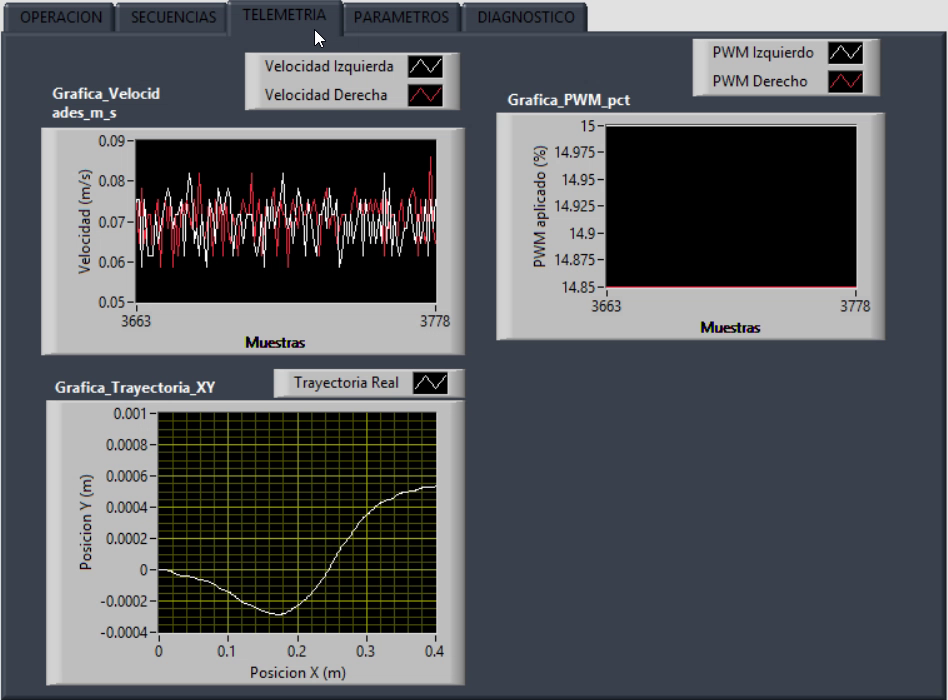
\includegraphics[width=\linewidth]{figures/ui_labview_telemetry.png}\caption{LabVIEW telemetry tab (myRIO).}\end{subfigure}
  \caption{Operator interfaces. The web page displays plate, ball, and drone status, a guided startup sequence, and a ``PARAR TODO'' (STOP ALL) button (also mapped to the spacebar); the LabVIEW panel shows wheel speeds, PWM, and the $x$--$y$ trajectory.}
  \label{fig:ui}
\end{figure}

\paragraph{Prerequisites}
\begin{itemize}
  \item charged batteries: both LiPo packs at \SI{12.6}{\volt} at rest and within \SI{0.05}{\volt} of each other, the NiMH pack, both 18650 packs, and the power bank;
  \item propellers inspected and tightened;
  \item vertical guide unobstructed, with both end-stops in place;
  \item a laptop or smartphone on the same Wi-Fi network as the Pi;
  \item two operators: one at the web page with the spacebar ready for immediate stop, and one watching the robot with the emergency stop (SB1) in hand;
  \item safety glasses for everyone within \SI{2}{\metre}.
\end{itemize}

\paragraph{Startup sequence}
Fig.~\ref{fig:fsm_dron} summarizes the octocopter firmware v11 state machine governing startup, guided flight, and safety cutoffs.
\begin{enumerate}
  \item With SB1 pressed, switch on logic power (SW1). \texttt{arrancar.sh} starts \texttt{seguidor.py} and restarts it if it exits. Wait for the NodeMCU to boot so the boot pulses emitted on GPIO5 and GPIO14 do not reach energized ESCs.
  \item Power on the myRIO and run the LabVIEW VI. The UART module must display the received ball position and drone angles (Fig.~\ref{fig:ui}b).
  \item On \texttt{/robot}:
  \begin{enumerate}[label=\alph*.]
    \item set the plate to ``Neutro'' (Neutral);
    \item with the drone level and still, click ``Calibrar'' (Calibrate) and wait \SI{5}{\second} until \texttt{CAL OK} appears;
    \item click ``Iniciar PID'' (Start PID) with the ball near the center.
  \end{enumerate}
  \item Measure and record the resting voltage of both LiPo packs, then connect them. Release SB1 (relays K1--K4 close). Click ``Armar e iniciar motores'' (Arm and start motors): the collective ramps up to \SI{1300}{\micro\second} (idle) and the attitude loop becomes active.
  \item \textbf{Bench mode} (moving base, drone at idle). Drive the base from LabVIEW using a manual command, a distance target, a \SI{360}{\degree} turn, go-to-point, or a loaded sequence.
  \item \textbf{Ramp mode} (proposed, Section~\ref{sec:porquedron}). Before the ramp, raise the collective with ``Subir'' (Up) to 1450--\SI{1550}{\micro\second} ($f\approx0.35$--0.55): the module remains seated while the rotors provide weight relief. Lower back to \SI{1300}{\micro\second} after clearing the climb. Above \SI{1500}{\micro\second}, the firmware limits the run to \SI{90}{\second}.
  \item \textbf{Guided flight.} Click ``Flotar'' (Hover): the collective ramps up at \SI{25}{\micro\second\per\second}, slowing to \SI{8}{\micro\second\per\second} above \SI{1650}{\micro\second}, up to \SI{1750}{\micro\second}. If the module does not lift off, click ``Subir'' ($+$\SI{25}{\micro\second}) and record the liftoff collective; if it exceeds \SI{1825}{\micro\second}, land and swap the batteries (Section~\ref{sec:bateria}). Use ``Subir''/``Bajar'' (Up/Down, $\pm$\SI{25}{\micro\second}) and ``Mantener'' (Hold); finish with ``Aterrizar'' (Land), which ramps down at \SI{60}{\micro\second\per\second}.
\end{enumerate}

\begin{figure}[!htbp]
\centering
\begin{tikzpicture}[font=\footnotesize, >=Latex,
  st/.style={draw, rounded corners=3pt, align=center, minimum height=11.5mm, inner xsep=3.5pt, inner ysep=3pt, line width=0.7pt},
  stOff/.style={st, draw=pGris!90!black, fill=pGris!12, line width=1.1pt, text width=2.80cm},
  stPre/.style={st, draw=pOcre, fill=pOcre!10, text width=2.55cm},
  stVis/.style={st, draw=pAzul, fill=pAzul!8, text width=2.65cm},
  stArm/.style={st, draw=pOcre, fill=pOcre!12, text width=2.45cm},
  stRmp/.style={st, draw=pAzul, fill=pAzul!10, text width=2.65cm},
  stSub/.style={st, draw=pVerde!90!black, fill=white, minimum height=15mm, text width=4.85cm},
  stCut/.style={st, draw=pRojo, fill=pRojo!8, align=left, text width=4.68cm, line width=0.85pt, inner xsep=3pt, inner ysep=2pt, font=\footnotesize\linespread{0.95}\selectfont},
  tr/.style={->, line width=0.8pt, pAzul!90!black, rounded corners=2.5pt},
  trG/.style={->, line width=0.8pt, pVerde!85!black, rounded corners=2.5pt},
  trR/.style={->, line width=0.95pt, pRojo, rounded corners=2.5pt},
  lbl/.style={font=\footnotesize, align=center, inner sep=1.5pt}]

  % ---- Level 1: Preparation (y = 0.00, total width 0.00..13.50 cm <= 13.74 cm)
  \node[stPre] (cal) at (1.42, 0.00) {\textbf{CAL}\\ \SI{5}{\second} still\\ (1000 samples)};
  \node[stOff] (off) at (6.75, 0.00) {\textbf{DISARMED}\\ (\texttt{OFF}, \SI{1000}{\micro\second})};
  \node[stVis] (vis) at (12.02, 0.00) {\textbf{PREVIEW}\\ (\texttt{vista},\\ \SI{1000}{\micro\second})};

  % Start arrow into DISARMED
  \fill[pGris!90!black] (6.75, 1.20) circle (0.08);
  \draw[->, thick, pGris!90!black] (6.75, 1.13) -- node[right=2pt]{\texttt{setup()}} (off.north);

  % Level 1 transitions (gaps 2.85..5.20 = 2.35 cm and 8.30..10.55 = 2.25 cm)
  \draw[tr]  ([yshift=2.4mm]off.west) -- node[lbl, above=1.5pt]{\texttt{cal} ($\ge\SI{4}{\second}$)} ([yshift=2.4mm]cal.east);
  \draw[tr]  ([yshift=-2.4mm]cal.east) -- node[lbl, below=1.5pt]{CAL OK\\ or rejected} ([yshift=-2.4mm]off.west);
  \draw[tr]  ([yshift=2.4mm]off.east) -- node[lbl, above=1.5pt]{\texttt{vista} (cal.)} ([yshift=2.4mm]vis.west);
  \draw[trR] ([yshift=-2.4mm]vis.west) -- node[lbl, below=1.5pt, pRojo]{\texttt{parar} / \texttt{!}} ([yshift=-2.4mm]off.east);

  % ---- Level 2: Safety (left), ARMED (center), RAMP (right) (y = -3.65)
  \node[stCut] (cut) at (2.48, -3.72) {%
    \textbf{\textcolor{pRojo}{Safety cutoffs}}\\
    $\bullet$ \texttt{parar}, \texttt{!}, or invalid cmd\\
    $\bullet$ tilt $\ge\SI{12}{\degree}$\\
    $\bullet$ yaw $\ge20^\circ$$^\ast$\\
    $\bullet$ yaw rate $\ge35^\circ$/s$^\ast$\\
    $\bullet$ I$^2$C or PWM error\\
    $\bullet$ slow IMU; loop $>\SI{30}{\milli\second}$\\
    {\scriptsize $^\ast$at idle: $\pm20^\circ$ window, $120^\circ$/s}};
  \node[stArm] (arm) at (7.45, -3.65) {\textbf{ARMED}\\ awaits \texttt{iniciar}\\ (\SI{10}{\second} timeout)};
  \node[stRmp] (rmp) at (12.02, -3.65) {\textbf{RAMP}\\ $1000\to\SI{1300}{\micro\second}$\\ ($+5\us/\SI{20}{\milli\second}$)};

  % Level 1 <-> Level 2 transitions (vertical space -0.65..-2.55)
  % DISARMED and PREVIEW share the arm BANCO_FIJO transition into ARMED
  \draw[tr]  ([xshift=7mm]off.south) -- node[lbl, right=2pt, pos=0.62, align=left]{\texttt{arm BANCO\_FIJO}\\ (cal., $\le\SI{4}{\degree}$, $\le\SI{5}{\degree\per\second}$)} (arm.north);
  \draw[tr]  (vis.south) -- ++(0,-0.48) -| ([xshift=7mm]off.south |- 0,-1.35);
  % 10 s timeout from ARMED to DISARMED (left of arm.north)
  \draw[trR] ([xshift=-8mm]arm.north) -- node[lbl, left=2pt, pos=0.52, pRojo]{\SI{10}{\second}} ([xshift=-1mm]off.south);
  % Exit from Safety cutoffs to DISARMED (clean label above elbow, well above cut.north)
  \draw[trR] ([xshift=19mm]cut.north) -- (4.38,-1.52) -| ([xshift=-10mm]off.south);
  \node[lbl, pRojo, left=3pt, align=right] at (4.34, -1.68) {\texttt{stop()} $\to\SI{1000}{\micro\second}$};
  % Stop from ARMED to Safety cutoffs
  \draw[trR] (arm.west) -- node[lbl, above=1.5pt, pRojo]{\texttt{parar}} (cut.east |- arm.west);
  % ARMED -> RAMP (gap 8.80..10.55 = 1.75 cm)
  \draw[tr]  (arm.east) -- node[lbl, above=1.5pt]{\texttt{iniciar}} node[lbl, below=1.5pt, align=center]{$<\SI{10}{\second}$\\ $\le\SI{4}{\degree}$} (rmp.west);

  % ---- Level 3: CONTROL container (y = -6.30..-13.25, width 0.00..13.50 cm)
  \node[stSub] (flt) at (2.82, -7.85) {\textbf{Hover / manual collective}\\ \texttt{flotar} (\SI{1750}{\micro\second}), \texttt{maximo} (\SI{1950}{\micro\second})\\ \texttt{subir}/\texttt{bajar} ($\pm\SI{25}{\micro\second}$); needs \texttt{hb}};
  \node[stSub] (ral) at (10.68, -7.85) {\textbf{Idle / base}\\ \SI{1300}{\micro\second}; $\pm\SI{20}{\degree}$ window\\ (yaw cutoff \SI{120}{\degree\per\second})};
  \node[stSub] (alt) at (2.82, -11.20) {\textbf{Altitude hold}\\ \texttt{mantener} ($\sigma<\SI{30}{\milli\metre}$)\\ Kalman + cascade $\pm\SI{60}{\micro\second}$\\ \texttt{subir}/\texttt{bajar} $\pm\SI{20}{\milli\metre}$};
  \node[stSub] (atr) at (10.68, -11.20) {\textbf{Land}\\ \texttt{aterrizar} $\to$ ramp $-\SI{60}{\micro\second\per\second}$\\ down to \SI{1300}{\micro\second}};

  % Automatic watchdogs note inside CONTROL (centered without forced justification)
  \node[font=\footnotesize, text=pVerde!75!black, align=center] (vig) at (6.75, -12.82)
    {Automatic watchdogs: no \texttt{hb} for \SI{1.5}{\second} or $>\SI{1500}{\micro\second}$ for \SI{90}{\second} $\to$ \SI{1300}{\micro\second};\\
     $>\SI{1850}{\micro\second}$ for \SI{20}{\second} $\to$ \SI{1750}{\micro\second}.};

  % CONTROL container frame on background layer
  \begin{scope}[on background layer]
    \node[draw=pVerde, fill=pVerde!6, rounded corners=4pt, line width=1pt,
          fit=(flt)(ral)(alt)(atr)(vig), inner xsep=6pt, inner ysep=8pt,
          yshift=3.8mm] (ctrl) {};
  \end{scope}
  \node[font=\footnotesize\bfseries, text=pVerde!85!black, anchor=north west]
    at ([xshift=5pt, yshift=-2.5pt]ctrl.north west) {CONTROL (\SI{200}{\hertz} attitude loop, collective 1300--\SI{1950}{\micro\second})};

  % RAMP -> CONTROL (Idle) entry (label to the right of the blue arrow, clear of the red arrow)
  \draw[tr] ([xshift=1mm]rmp.south) -- (ral.north -| 12.12,0);
  \node[lbl, right=2pt, align=left] at (12.15, -5.00) {\SI{1300}{\micro\second}\\ (\SI{1.2}{\second})};

  % Internal transitions inside CONTROL (ample vertical space -8.70..-10.35)
  \draw[trG] (ral.west) -- node[lbl, above=1.5pt]{\texttt{flotar}, \texttt{subir}} node[lbl, below=1.5pt]{(with \texttt{hb})} (flt.east);
  \draw[trG] ([xshift=-4mm]flt.south) -- node[lbl, left=2pt, align=right]{\texttt{mantener}\\ ($\sigma<\SI{30}{\milli\metre}$)} ([xshift=-4mm]alt.north);
  \draw[trG] ([xshift=6mm]alt.north) -- node[lbl, right=2pt, align=left]{other cmd or\\ laser $>\SI{2}{\second}$} ([xshift=6mm]flt.south);
  \draw[trG] ([yshift=-4mm]flt.east) -- (5.80,-8.25) |- ([yshift=2mm]atr.west);
  \node[lbl, text=pVerde!85!black, above=1.5pt, align=center] at (7.00,-11.00) {\texttt{aterrizar} /\\ watchdog};
  \draw[trG] ([yshift=-2.5mm]alt.east) -- ([yshift=-2.5mm]atr.west);
  \draw[trG] (atr.north) -- node[lbl, right=2pt]{reaches \SI{1300}{\micro\second}} (ral.south);

  % Safety exits from RAMP and CONTROL to Safety cutoffs (in open corridor -5.65)
  \draw[trR] ([xshift=-10mm]rmp.south) -- (11.02,-5.68) -| ([xshift=14mm]cut.south);
  \draw[trR] (ctrl.north -| 2.15,0) -- node[lbl, left=2pt, pRojo]{cutoff / \texttt{parar}} (cut.south -| 2.15,0);
\end{tikzpicture}
\vspace{-4pt}
\caption{\raggedright Octocopter firmware v11 state machine (\texttt{captura\_octo\_m8\_vuelo\_guia.ino}). Transition functions: boot to \texttt{DISARMED} (\texttt{setup()}); serial commands \texttt{cal}, \texttt{vista}, \texttt{arm BANCO\_FIJO}, \texttt{iniciar}, \texttt{flotar}, \texttt{maximo}, \texttt{subir}, \texttt{bajar}, \texttt{mantener}, \texttt{aterrizar}, \texttt{parar}, and rejected command (\texttt{command()}); \texttt{!} stop and invalid line (\texttt{serialInput()}); calibration end (\texttt{collectCalibration()}); \SI{10}{\second} timeout in \texttt{ARMED}, \texttt{RAMP} to \texttt{CONTROL} (\SI{1300}{\micro\second}), and MCPWM fault (\texttt{loop()}); collective and \texttt{hb} heartbeat (\texttt{fijarObjetivo()}, \texttt{hbReciente()}); collective ramp, altitude hold, and watchdogs (\SI{1.5}{\second}, \SI{20}{\second}, \SI{90}{\second}, and \SI{2}{\second} without laser; \texttt{actualizarColectivo()}); attitude/yaw cutoffs (\texttt{checkAttitudeCutoff()}); and I$^2$C error, IMU $>\SI{15}{\milli\second}$, or late loop (\texttt{imuFault()} from \texttt{loop()}). Every cutoff calls \texttt{stop()} (\SI{1000}{\micro\second}, \texttt{DISARMED}).}
\label{fig:fsm_dron}
\end{figure}

\paragraph{Reading results}
Each run produces three logs:
\begin{itemize}
  \item \texttt{registros/registro\_*.csv}: ball position, servo pulses, and status at the camera frame rate;
  \item \texttt{registros/vuelo\_*.csv}: drone attitude, motor commands, accelerometer, laser range, and collective at \SI{10}{\hertz};
  \item the drone onboard buffer (last \SI{16}{\second} at \SI{100}{\hertz}, 1600 samples), exported via ``Exportar registro'' (Export log).
\end{itemize}
The scripts in \texttt{analysis/} compute the metrics reported in Section~\ref{sec:validation}. Record the resting LiPo voltage before and \SI{10}{\minute} after each flight, along with each video timestamp, so videos can be cross-referenced with the logs as in Section~\ref{sec:flights}.

\paragraph{Operating limits and protections}
Drone firmware v11 stops the motors in five cases:
\begin{itemize}
  \item estimated tilt exceeds \SI{12}{\degree};
  \item above \SI{1400}{\micro\second} (or with base yaw rate \texttt{yb} active), relative yaw exceeds \SI{20}{\degree} or relative yaw rate exceeds \SI{35}{\degree\per\second};
  \item at idle on the base ($\le\SI{1400}{\micro\second}$, without \texttt{yb}), the heading reference slides within a $\pm\SI{20}{\degree}$ window without angle cutoff, while a \SI{120}{\degree\per\second} rate cutoff remains active;
  \item the estimated IMU state becomes non-finite;
  \item any unknown command arrives.
\end{itemize}
It also limits the collective in three situations:
\begin{itemize}
  \item without the Pi heartbeat (\texttt{hb}, sent every \SI{0.3}{\second}), the collective is capped at \SI{1400}{\micro\second}, and after \SI{1.5}{\second} without a heartbeat it drops to \SI{1300}{\micro\second};
  \item above \SI{1850}{\micro\second}, the collective returns to \SI{1750}{\micro\second} after \SI{20}{\second} to protect the \SI{30}{\ampere} fuses;
  \item above \SI{1500}{\micro\second}, the collective drops after \SI{90}{\second}.
\end{itemize}
The firmware does not measure battery voltage. With charged LiPo packs, useful continuous hover time is 3--\SI{7}{\minute} (Section~\ref{sec:bateria}); keep runs short and do not discharge LiPo packs below \SI{11.1}{\volt} at rest (\SI{3.7}{\volt} per cell).

\paragraph{Safe shutdown}
\begin{enumerate}
  \item Click ``Aterrizar'' (Land) and wait for the collective to reach \SI{1300}{\micro\second}; then click ``Parar'' (Stop).
  \item Set the plate to ``Neutro'' (Neutral) and stop the base.
  \item Press SB1 and disconnect the LiPo batteries before touching the drone.
  \item Export the logs and record the resting LiPo voltage.
\end{enumerate}
In an emergency, press the spacebar (all motors stop immediately and the drone drops onto the lower end-stop) and press the emergency stop (SB1), which simultaneously disconnects both LiPo branches, the mobile base, and the servos.

\subsection{Basic troubleshooting}
\label{sec:troubleshooting}
Table~\ref{tab:troubleshooting} summarizes faults observed during prototype testing, their probable causes, and recommended actions.

\begin{table}[!htbp]
\centering
\caption{Basic troubleshooting for faults observed during AeroTray operation.}
\label{tab:troubleshooting}
\footnotesize
\begin{tabularx}{\textwidth}{@{}>{\raggedright\arraybackslash}p{0.27\textwidth}>{\raggedright\arraybackslash}p{0.31\textwidth}>{\raggedright\arraybackslash}X@{}}
\toprule
Symptom & Probable cause & Recommended action \\
\midrule
\texttt{ORDEN RECHAZADA} or \texttt{CAL RECHAZADA} when calibrating & IMU did not initialize after flashing or rebooting the NodeMCU (\texttt{IMU=0} at boot) & Press EN on the NodeMCU, wait \SI{5}{\second}, and calibrate with the drone still and level \\
Web page unresponsive or Pi not visible & Laptop or Pi switched networks & Connect both to the same hotspot and locate the Pi by its MAC address \\
Servos receive pulses but the plate does not move & Missing servo power (BT6, regulator, or common ground) & Check BT6, the XL4015 at \SI{5.2}{\volt}, and the common ground with the ESP32-S3 \\
Laser reports \texttt{estado 2} or invalid readings & Weak return signal from the floor & Place the white target sheet under the sensor; the firmware uses long-range mode with filtering \\
Ball is not detected & Lighting or color & Control ambient lighting; inspect the ``Cámara'' (Camera) view on \texttt{/robot} \\
\texttt{Flotar} does not lift off & Discharged LiPo packs ($<\SI{12.4}{\volt}$ at rest) & Measure and charge the LiPo packs; at \SI{11.1}{\volt} the module cannot lift off below the sustained limit \\
Tilt (\SI{12}{\degree}) or yaw cutoff & Impact at a ramp break or base rotation with collective $>\SI{1400}{\micro\second}$ & Recalibrate and re-arm; cross the ramp at idle \\
\bottomrule
\end{tabularx}
\end{table}
